\documentclass[cn,11pt,chinese]{elegantbook}

\usepackage[all]{xy}
\usepackage{amsmath}
\usepackage{asymptote}
\usepackage{subfig}
\usepackage{graphicx}



\newcount\mycount
\def\cis{\,\text{cis}\,}
\def\intset{\operatorname{int}}
\def\diam{\operatorname{diam}}
\def\dist{\operatorname{dist}}
\def\ulim{\operatorname{u-lim}}
\def\cinfty{\mathbb{C}_{\infty}}
\def\sh{\operatorname{sh}}
\def\argsh{\operatorname{argsh}}
\def\ch{\operatorname{ch}}
\def\argch{\operatorname{argch}}
\def\real{\mathbb{R}}
\def\dsint{{\displaystyle\int}}

\numberwithin{equation}{section}


% title info
\title{微积分}
\subtitle{第一卷}

% bio info
\author{Tom. M. Apostol}

% extra info
\version{1.00}
\extrainfo{Wir m\"ussen wissen, wir werden wissen. (我们必须知道,我们必将知道) - David.Hilbert}
%\logo{logo.png}
\cover{cover.jpg}

\begin{document}


\maketitle

\chapter*{Preface}


\tableofcontents
\mainmatter
\hypersetup{pageanchor=true}

% add preface chapter here if needed

\chapter{Introduction}
\section{Historical Introduction}

\subsection{The two basic concepts of calculus}
The remarkable progress that has been made in science and technology during the last Century is due in large part to the development of mathematics. That branch of mathematics known as integral and differential calculus serves as a natural and powerful tool for attacking a variety of problems that arise in physics, astronomy, engineering, chemistry, geology, biology, and other fields including, rather recently, some of the social sciences.

To give the reader an idea of the many diffrent types of problems that can be treated by the methods of calculus, we list here a few sample questions selected from the exercises that occur in later chapters of this book.

With what speed should a rocket be fired upward so that it never returns to earth?What is the radius of the smallest circular disk that can cover every isosceles triangle of a given perimeter $L$? What volume of material is removed from a solid sphere of radius $2r$ if a hole of radius $r$ is drilled through the center? If a strain of bacteria grows at a rate proportional to the amount present and if the population doubles in one hour, by how much will it increase at the end of two hours? If a ten-pound force stretches an elastic spring one inch, how much work is required to stretch the spring one foot? 

These examples, chosen from various fields, illustrate some of the technical questions that can be answered by more or less routine applications of calculus.

Calculus is more than a technical tool --- it is a collection of fascinating and exciting ideas that have interested thinking men for centuries. These ideas have to do with speed, area, volume, rate of growth, continuity, tangent line, and other concepts from a variety of fields. Calculus forces us to stop and think carefully about the meanings  of these concepts. Another remarkable feature of the subject is its unifying power. Most of these ideas can be formulated so that they revolve around two rather specialized problems of a geometric nature. We turn now to a brief description of these problems.

Consider a curve $C$ which lies above a horizontal base line such as that shown in Figure 1.1. We assume this curve has the property that every vertical line intersects it once at most. The shaded portion of the figure consists of those points which lie below the curve $C$, above the horizontal base, and between two parallel vertical segments joining $C$ to the base. The first fundamental problem of calculus is this: To assign a number which measures the area of this shaded region.

Consider next a line drawn tangent to the curve, as shown in  Figure 1.1. The second fundamental problem may be stated as follow: To assign a number which measures the steepness of this line.

Basically, calculus has to do with the precise formulation and solution of these two special problems. It enables us to define the concepts of area and tangent line and to calculate the area of a given region or the steepness of a given tangent line. Untegral calculus deals with the problem of area and will be discussed in Chapter 1. Differential calculus deals with the problem of tangents and will be introduced in Chapter 4.

The study of calculus requires a certain mathematical background. The present chapter deals with this background material and is divided into four parts: Part 1 provides historical perspective; Part 2 discusses some notation and terminology from the mathematics sets; Part 3 deals with the real-number system; Part 4 treats mathematical induction and the summation notation. If the reader is acquainted with these topics, ha can proceed directly to the developmentof intergral calculus in Chapter 1. If not, he should become familiar with the material in the unstarred sections of this Introduction before proceeding to Chapter 1.

\subsection{Historical background}
The birth of integral calculus occurred more than 2000 years ago when the Greeks attemplted to determine areas by a process which they called the method of exhaustion. The essential ideas of this method are very simple and can be described briefly as follows: Given a region whose area is to be determined, we inscribe in it a polygonal region which approximates the given region and whose area we easily compute. Then we choose another polygonal region which gives a better approximation, and we continue the process, taking polygons with more and more sides in an attemplt to exhaust the given region. The method is illustrated for a semicircular region in Figure 1.2. It was used successfully by Archimedes (287 -212 B.C.) to find exact formulas for the area of a circle and a few other special figures.

The development of the method of exhaustion beyond the point to which Archimedes carried it has to wait nearly eighteen centuries until the use of algebraic symbols and techniques bacame a standard part of mathematics. The elementary algebra that is familiar to most high-school students today was completely unknown in Archimedes' time, and it would have been next to impossible to extend his method to any general class of regions without some convenient way of expressing rather lengthy calculations in a compact and simplified form.

A slow but revolutionary change in the development of mathematical notations began in the 16th century A.D. The cumbersome system of Roman numerals was gradually dispalced by the Hindu-Arabic characters used today, the symbols $+$ and $-$ were introduced for the first time, and the advantages of the decimal notation began to be recognized. During this same period, the brilliant successes of the Italian mathematicians Tartaglia, Cardano, and Ferrari in finding algebraic solutions of cubic and quartic equations stimulated a greatdeal of activity in mathematics and encouraged the growth and acceptance of a new superior algebraic language. With the widespread introduction of well-chosen algebraic symbols, interest was revived in the ancient method of exhaustion and a large number of fragmentary results were discovered in the 16th century by such pioneers as Cavalieri, Toricelli, Roberval, Fermat, Pascal, and Wallis.

Gradually the method of exhaustion was transformed into the subject now called integral calculus, a new and powerful discipline with a large variety of applications, not only to geometrical problems concerned with areas and volumes but also to problems in other sciences. This branch of mathematics, which retained some of the original features of the method of exhaustion, received its biggest impetus in the 17th century, largely due to the efforts of Isaac Newton (1642-1727) and Gottfried Leibniz (1646-1716), and its development continued well into the 19th century before the subject was put on a firm mathematical basis by such men as Augustin-Louis Cauchy (1789-1857) and Bernhard Riemann (1826-1866). Further refinements and extensions of the theory are still being carried out in contemporary mathematics.

\subsection{The method of exhaustion for the area of a parabolic segment}
Before we proceed to a systematic treatment of integral calculus, it will be







% \bibliographystyle{plain}
\bibliography{mathreference}
\appendix
% h
\chapter{Tikz绘制的一些图形}
\begin{center}
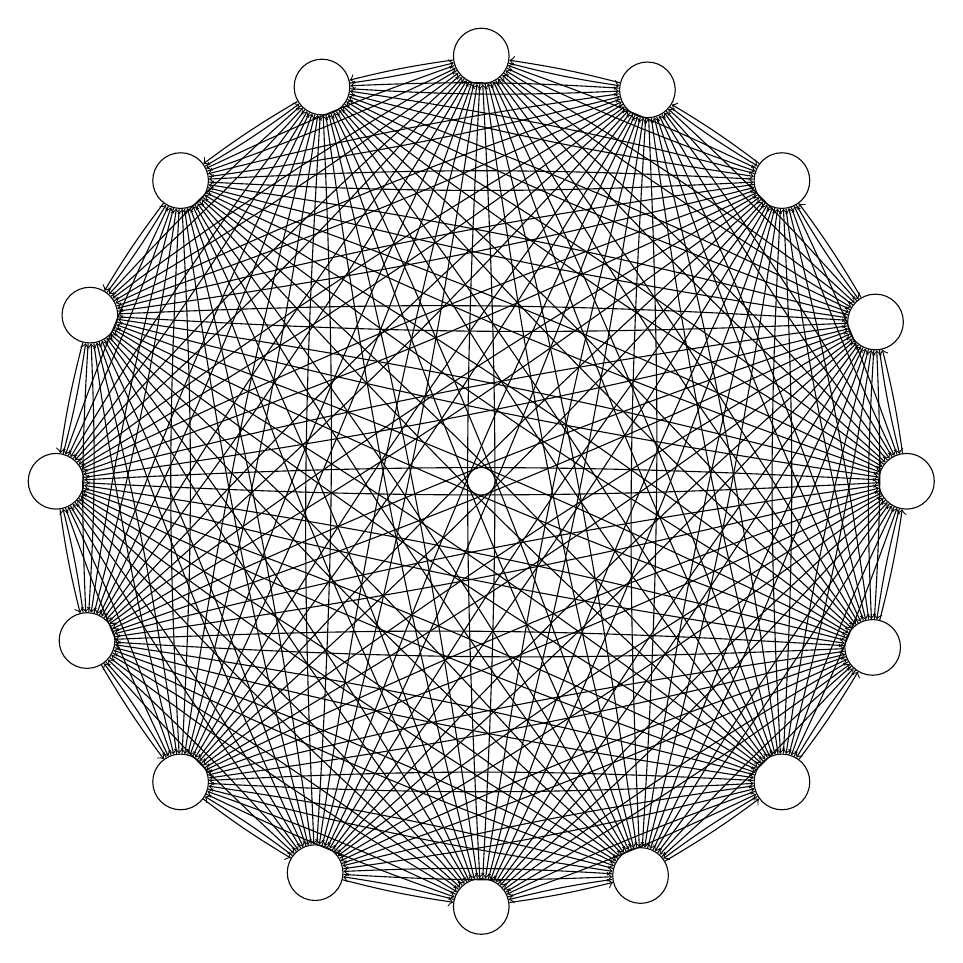
\begin{tikzpicture}[transform shape]
  %the multiplication with floats is not possible. Thus I split the loop in two.
  \foreach \number in {1,...,8}{
      % Computer angle:
        \mycount=\number
        \advance\mycount by -1
  \multiply\mycount by 45
        \advance\mycount by 0
      \node[draw,circle,inner sep=0.25cm] (N-\number) at (\the\mycount:5.4cm) {};
    }
  \foreach \number in {9,...,16}{
      % Computer angle:
        \mycount=\number
        \advance\mycount by -1
  \multiply\mycount by 45
        \advance\mycount by 22.5
      \node[draw,circle,inner sep=0.25cm] (N-\number) at (\the\mycount:5.4cm) {};
    }
  \foreach \number in {1,...,15}{
        \mycount=\number
        \advance\mycount by 1
  \foreach \numbera in {\the\mycount,...,16}{
    \path (N-\number) edge[->,bend right=3] (N-\numbera)  edge[<-,bend
      left=3] (N-\numbera);
  }
}
\end{tikzpicture}


\begin{tikzpicture}
 \definecolor{r1}{RGB}{0,129,188}
 \definecolor{r2}{RGB}{252,177,49}
 \definecolor{r3}{RGB}{35,34,35}
 \definecolor{r4}{RGB}{0,157,87}
 \definecolor{r5}{RGB}{238,50,78}
 \begin{scope}
   \clip (-6,2) rectangle (6,-.9);
   \foreach \col/\xp/\yp in {
     r5/4/0, r4/2/-1.8, r3/0/0,
     r2/-2/-1.8, r1/-4/0
   } {
     \path[draw=white,line width=.08cm,
     fill=\col,even odd rule]
     (\xp, \yp) circle (1.9cm)
     (\xp, \yp) circle (1.5cm);
   }
 \end{scope}
 \begin{scope}
   \clip (-6,-.9) rectangle (6,-3.8);
   \foreach \col/\xp/\yp in {
     r1/-4/0, r2/-2/-1.8, r3/0/0,
     r4/2/-1.8, r5/4/0
   } {
     \path[draw=white,line width=.08cm,
     fill=\col,even odd rule]
     (\xp, \yp) circle (1.9cm)
     (\xp, \yp) circle (1.5cm);
   }
 \end{scope}
\end{tikzpicture}


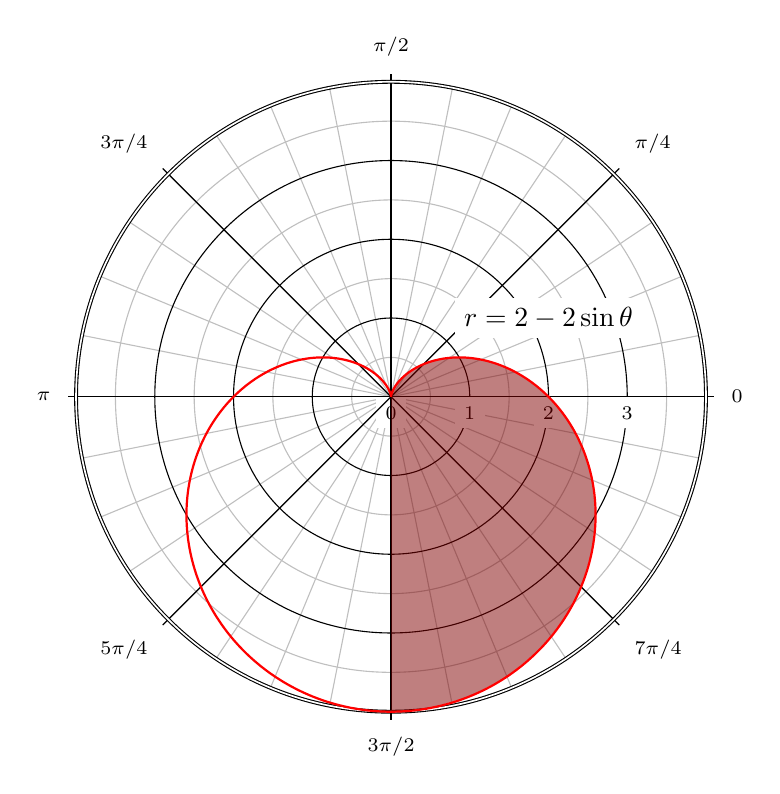
\begin{tikzpicture}[>=latex]

% Draw the lines at multiples of pi/12
\foreach \ang in {0,...,31} {
  \draw [lightgray] (0,0) -- (\ang * 180 / 16:4);
}

% Concentric circles and radius labels
\foreach \s in {0, 1, 2, 3} {
  \draw [lightgray] (0,0) circle (\s + 0.5);
  \draw (0,0) circle (\s);
  \node [fill=white] at (\s, 0) [below] {\scriptsize $\s$};
}

% Add the labels at multiples of pi/4
\foreach \ang/\lab/\dir in {
  0/0/right,
  1/{\pi/4}/{above right},
  2/{\pi/2}/above,
  3/{3\pi/4}/{above left},
  4/{\pi}/left,
  5/{5\pi/4}/{below left},
  7/{7\pi/4}/{below right},
  6/{3\pi/2}/below} {
  \draw (0,0) -- (\ang * 180 / 4:4.1);
  \node [fill=white] at (\ang * 180 / 4:4.2) [\dir] {\scriptsize $\lab$};
}

% The double-lined circle around the whole diagram
\draw [style=double] (0,0) circle (4);

\fill [fill=red!50!black, opacity=0.5] plot [domain=-pi/2:pi/2]
  (xy polar cs:angle=\x r, radius= {2-2*sin(\x r)});
\draw [thick, color=red, domain=0:2*pi, samples=200, smooth]
  plot (xy polar cs:angle=\x r, radius={2-2*sin(\x r)});
\node [fill=white] at (2,1) {$r=2-2\sin\theta$};

\end{tikzpicture} 


% definition de partial ellipse
\tikzset{partial ellipse/.style args =
  {#1:#2:#3}{insert path={+ (#1:#3) arc (#1:#2:#3)}}}
\begin{tikzpicture}[>=latex]
  %  ellipses
  \draw [fill=white!90!red]    (3,-1.8) ellipse    (4cm and 1 cm);
  \draw [fill=yellow!90!green] (3,-1.8) ellipse (3cm and 0.75 cm);
  \draw [fill=white!90!green]  (3,-1.8) ellipse  (2cm and 0.5 cm);

  % -- Soleil
  \shade [ball color=gray!10!yellow] (3,-1.8) circle (1);
  \node (soleil) at (3,-1.8) {\bf Soleil};
  % partial ellipse pour tracé devant le Soleil
  \draw (3,-1.8) [partial ellipse=220:320:2cm and 0.5cm]
        (3,-1.8) [partial ellipse=220:320:3cm and 0.75cm];

  % Venus
  \shade [ball color=gray!10!orange] (1.6,-1.8) circle (.2);
  \node (venus) at (1.5,-1.45) {Venus}; 

  % ombre de Venus
  \draw[color=white!70!black,fill=white!70!black]
    (1.6,-2.3) ellipse (2mm and 0.5mm);

  % Mercure
  \shade [ball color=gray!10!orange] (5,-1.225) circle (.25);
  \node (mercure) at (5,-0.8) {Mercure}; 

  % Earth
  \shade [ball color=white!50!blue] (5.75,-2.5) circle (.33);
  \node (terre) at (6.6,-2.6) {\bf Terre};

  % Lune
  \shade [ball color=yellow] (5.25,-2.8) circle (.1);
  \node (lune) at (5.25,-3) {Lune};
     
  % Mars
  \draw (3,-1.8) [partial ellipse=45:120:9cm and 2.5cm];
  \shade [ball color=black!50!red] (5,0.66) circle (.15);
  \node (mars) at (5,1) {\bf Mars};   
  % trajet
  \draw [line width=2pt,blue,->,>=latex] (terre) to[out=0,in=0] (mars);   
\end{tikzpicture}
\end{center}


\end{document}
